\chapter{p4 = 6 (4 graphs)}
\newpage\begin{figure}
  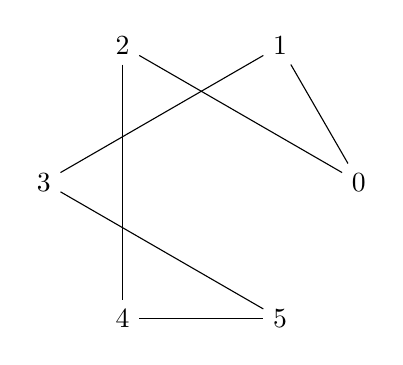
\begin{tikzpicture}
      \draw
        (0.0:2) node (0){0}
        (60.0:2) node (1){1}
        (120.0:2) node (2){2}
        (180.0:2) node (3){3}
        (240.0:2) node (4){4}
        (300.0:2) node (5){5};
      \begin{scope}[-]
        \draw (0) to (1);
        \draw (0) to (2);
        \draw (1) to (3);
        \draw (2) to (4);
        \draw (3) to (5);
        \draw (4) to (5);
      \end{scope}
    \end{tikzpicture}
\end{figure}
\begin{itemize}
\item signature: 110000100010011
\item g: Graph with 6 nodes and 6 edges
\item order: 6
\item size: 6
\item max degree: 2
\item degrees: 2,2,2,2,2,2
\item is tree: 0
\item is bipartite: 1
\item has bridge: 0
\item is chordal: 0
\item is complete: 0
\item min cycle basis weight: 6
\item min cycle basis size: 1
\item diameter: 3
\item radius: 3
\item is eulerian: 1
\item is planar: 1
\item number of faces: 2
\item is regular: 1
\item p3: 6
\item p4: 6
\item property hash: 94e71ef635553dbba82fb825ffbdb92681a82d9cce7ea578be96221a77303a54
\end{itemize}
\newpage
\begin{figure}
  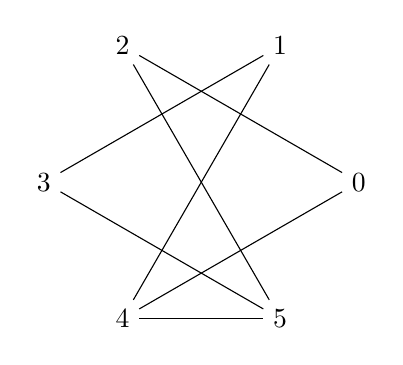
\begin{tikzpicture}
      \draw
        (0.0:2) node (0){0}
        (60.0:2) node (1){1}
        (120.0:2) node (2){2}
        (180.0:2) node (3){3}
        (240.0:2) node (4){4}
        (300.0:2) node (5){5};
      \begin{scope}[-]
        \draw (0) to (2);
        \draw (0) to (4);
        \draw (1) to (3);
        \draw (1) to (4);
        \draw (2) to (5);
        \draw (3) to (5);
        \draw (4) to (5);
      \end{scope}
    \end{tikzpicture}
\end{figure}
\begin{itemize}
\item signature: 010100110001011
\item g: Graph with 6 nodes and 7 edges
\item order: 6
\item size: 7
\item max degree: 3
\item degrees: 2,2,2,2,3,3
\item is tree: 0
\item is bipartite: 1
\item has bridge: 0
\item is chordal: 0
\item is complete: 0
\item min cycle basis weight: 8
\item min cycle basis size: 2
\item diameter: 3
\item radius: 2
\item is eulerian: 0
\item is planar: 1
\item number of faces: 3
\item is regular: 0
\item p3: 10
\item p4: 6
\item property hash: 0d37d15d2bdb8275d94a0f9aeca55ae56316027f7435ade215e6ecbc01bd531f
\end{itemize}
\newpage
\begin{figure}
  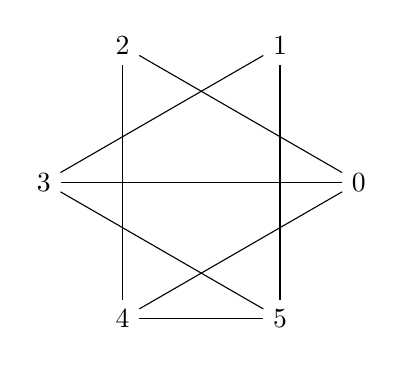
\begin{tikzpicture}
      \draw
        (0.0:2) node (0){0}
        (60.0:2) node (1){1}
        (120.0:2) node (2){2}
        (180.0:2) node (3){3}
        (240.0:2) node (4){4}
        (300.0:2) node (5){5};
      \begin{scope}[-]
        \draw (0) to (2);
        \draw (0) to (3);
        \draw (0) to (4);
        \draw (1) to (3);
        \draw (1) to (5);
        \draw (2) to (4);
        \draw (3) to (5);
        \draw (4) to (5);
      \end{scope}
    \end{tikzpicture}
\end{figure}
\begin{itemize}
\item signature: 011100101010011
\item g: Graph with 6 nodes and 8 edges
\item order: 6
\item size: 8
\item max degree: 3
\item degrees: 2,2,3,3,3,3
\item is tree: 0
\item is bipartite: 0
\item has bridge: 0
\item is chordal: 0
\item is complete: 0
\item min cycle basis weight: 10
\item min cycle basis size: 3
\item diameter: 3
\item radius: 2
\item is eulerian: 0
\item is planar: 1
\item number of faces: 4
\item is regular: 0
\item p3: 8
\item p4: 6
\item property hash: f3a6df97b34c34621f3f21cfa59b00ecf9d13fe7b47135f9aa1d731b58779ead
\end{itemize}
\newpage
\begin{figure}
  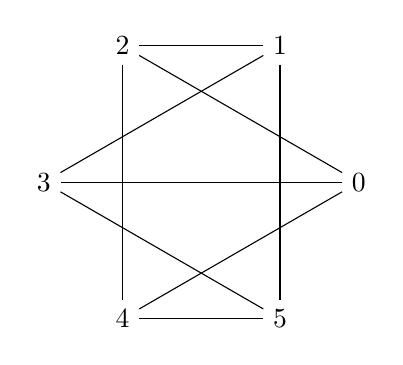
\begin{tikzpicture}
      \draw
        (0.0:2) node (0){0}
        (60.0:2) node (1){1}
        (120.0:2) node (2){2}
        (180.0:2) node (3){3}
        (240.0:2) node (4){4}
        (300.0:2) node (5){5};
      \begin{scope}[-]
        \draw (0) to (2);
        \draw (0) to (3);
        \draw (0) to (4);
        \draw (1) to (2);
        \draw (1) to (3);
        \draw (1) to (5);
        \draw (2) to (4);
        \draw (3) to (5);
        \draw (4) to (5);
      \end{scope}
    \end{tikzpicture}
\end{figure}
\begin{itemize}
\item signature: 011101101010011
\item g: Graph with 6 nodes and 9 edges
\item order: 6
\item size: 9
\item max degree: 3
\item degrees: 3,3,3,3,3,3
\item is tree: 0
\item is bipartite: 0
\item has bridge: 0
\item is chordal: 0
\item is complete: 0
\item min cycle basis weight: 14
\item min cycle basis size: 4
\item diameter: 2
\item radius: 2
\item is eulerian: 0
\item is planar: 1
\item number of faces: 5
\item is regular: 1
\item p3: 12
\item p4: 6
\item property hash: 51f8faee6f7c17cd9ca845af60a5f539872c53e9bcc8921a944032656f107bdc
\end{itemize}
\newpage
